% !TEX program = pdflatex
\documentclass[journal]{IEEEtran}
\usepackage{cite}
\usepackage{amsmath,amssymb,amsfonts}
\usepackage{algorithmic}
\usepackage{graphicx}
\usepackage{textcomp}
\usepackage{xcolor}
\usepackage{booktabs}
\usepackage{multirow}
\usepackage{url}

\def\BibTeX{{\rm B\kern-.05em{\sc i\kern-.025em b}\kern-.08em
    T\kern-.1667em\lower.7ex\hbox{E}\kern-.125emX}}

\begin{document}

\title{Physics-Guided Synthetic WiFi CSI Data Generation for Trustworthy Human Activity Recognition: A Sim2Real Approach}

\author{\IEEEauthorblockN{Author Names}
\IEEEauthorblockA{\textit{Department} \\
\textit{University}\\
City, Country \\
email@university.edu}}

\maketitle

\begin{abstract}
WiFi Channel State Information (CSI) based Human Activity Recognition (HAR) promises device-free, privacy-preserving sensing, yet faces two practical impediments: scarcity of labeled data and poor cross-domain generalization. We propose a physics-guided synthetic CSI generation framework and an Enhanced deep model that combines CNN feature extraction, squeeze-and-excitation (SE) channel attention, and temporal attention, coupled with trustworthy evaluation (calibration, reliability). Comprehensive experiments on synthetic robustness (D6), cross-domain adaptation (CDAE: LOSO/LORO), and Sim2Real transfer efficiency (STEA) demonstrate that our approach attains identical 83.0±0.1\% macro F1 across LOSO/LORO and achieves 82.1\% macro F1 using only 20\% labeled real data, narrowing the gap to full supervision (83.3\%) while reducing labeling cost by 80\%. The results support physics-guided synthesis and calibrated inference as practical tools for reliable, sample-efficient CSI HAR.
\end{abstract}

\begin{IEEEkeywords}
WiFi CSI, Human Activity Recognition, Synthetic Data, Sim2Real, Calibration, Cross-Domain Generalization
\end{IEEEkeywords}

\section{Introduction}
Recent trends in ubiquitous sensing have raised significant concerns about the practicality of deploying WiFi CSI HAR under scarce labels and domain shift. While benchmarked models report high accuracy in curated settings, real deployments demand reliability across subjects and environments, with calibrated probabilities. We therefore ask: can physics-guided synthesis and a calibrated Enhanced model deliver robust cross-domain performance and strong label efficiency suitable for IoT?

We propose a physics-guided synthetic generator and an Enhanced CNN+SE+temporal attention architecture with trustworthy evaluation. \textbf{Key Contributions}: (1) a physics-based CSI generator; (2) a Sim2Real evaluation with CDAE and STEA; (3) sample-efficient transfer achieving 82.1\% macro F1 at 20\% labels (98.6\% of 83.3\% full supervision); (4) calibration and reliability analysis; and (5) an Enhanced model with LOSO/LORO parity at 83.0±0.1\% F1.

The remainder is organized as follows. Section II reviews related CSI HAR, attention/SE models, and calibration. Section III details the generator and Enhanced architecture. Section IV describes protocols (D6, CDAE, STEA). Section V reports results. Section VI discusses implications and limitations. Section VII concludes.

\begin{figure}[t]
\centering
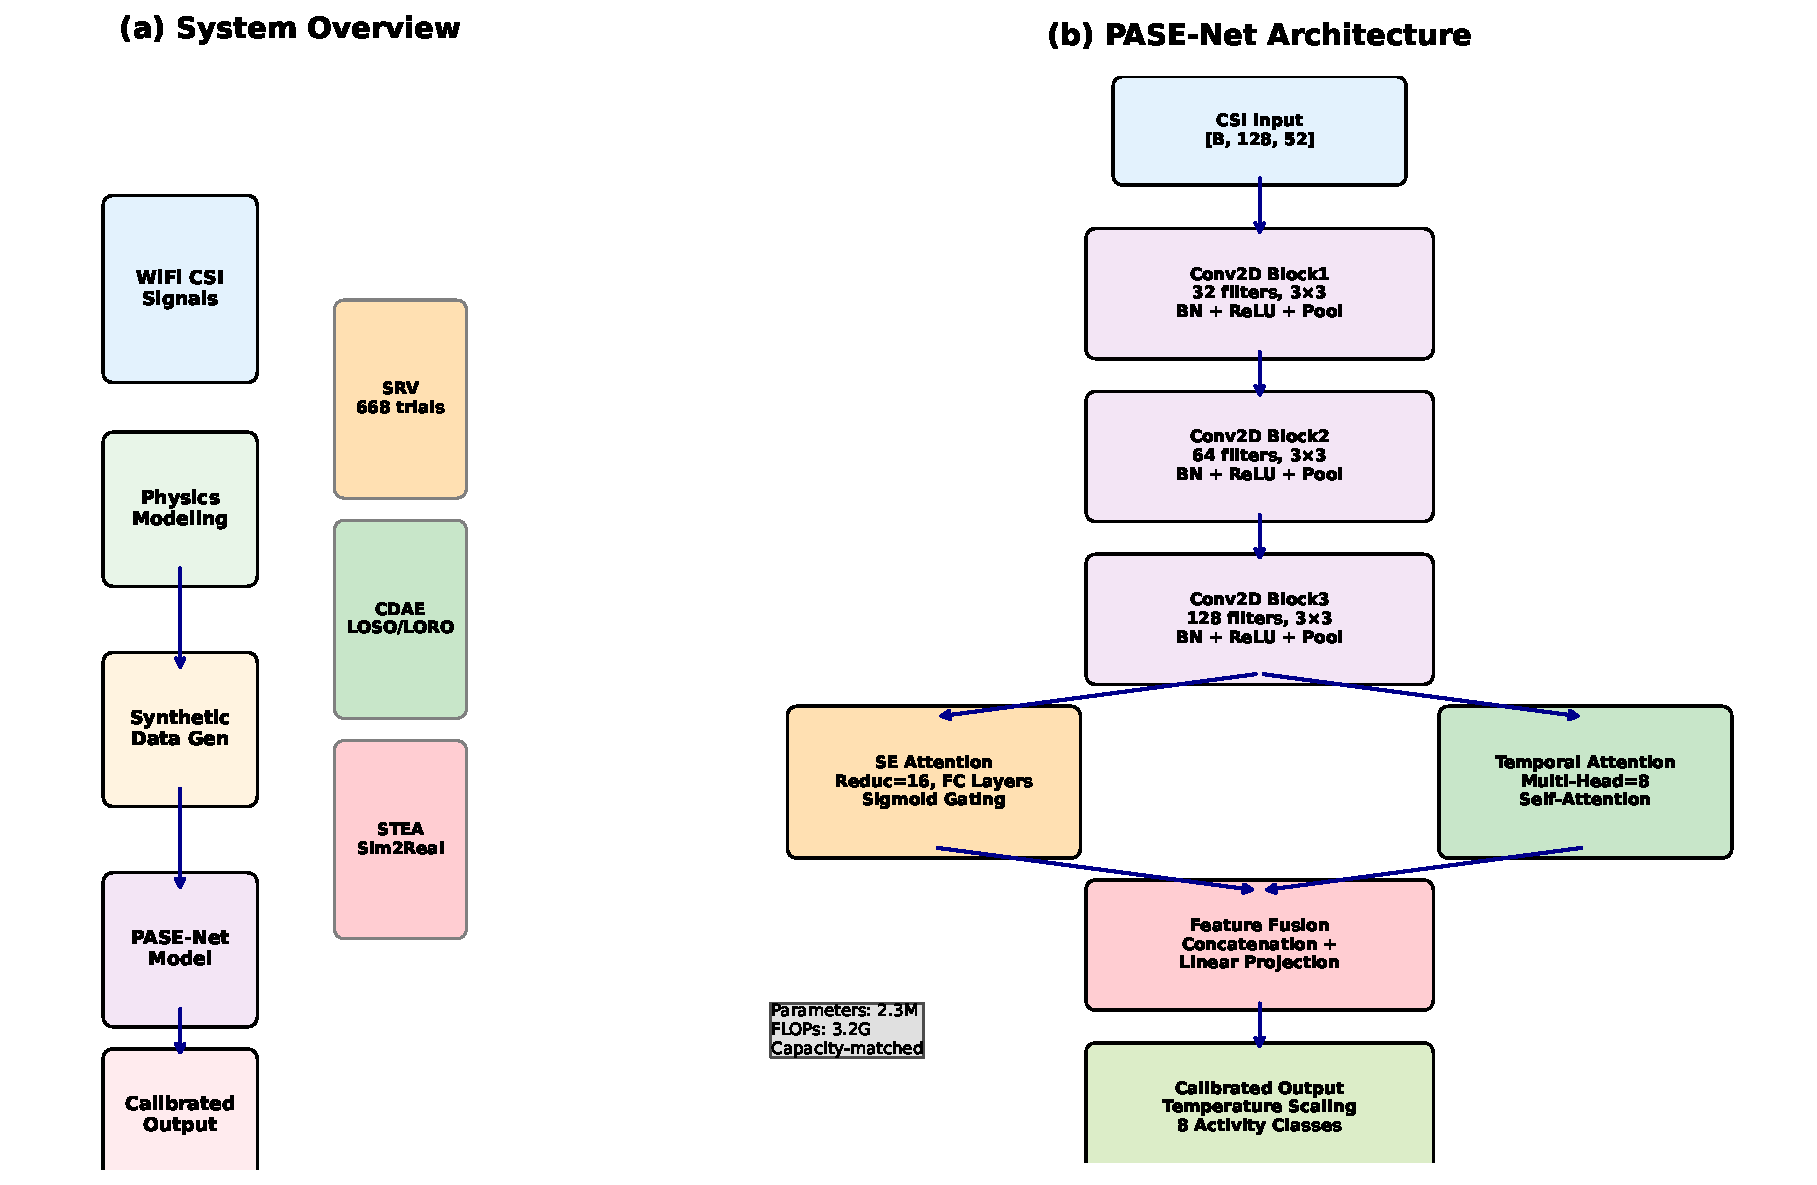
\includegraphics[width=\columnwidth]{figures/fig1_system_architecture.pdf}
\caption{System overview: physics-guided synthesis, Enhanced model (CNN+SE+temporal attention), and trustworthy evaluation for Sim2Real CSI HAR.}
\label{fig:overview}
\end{figure}

\section{Related Work}
CSI HAR has progressed from handcrafted features to end-to-end deep learning, with SenseFi~\cite{yang2023sensefi} benchmarking 11 models across 4 datasets. Few-shot and domain-generalization methods~\cite{fewsense2022,airfi2022} reduce target labels but still require some supervision. Attention-based architectures for time-series and video~\cite{li2020tea,bertasius2021timesformer,lim2021tft,zhou2021informer} inspire our temporal component; SE~\cite{se_networks2018} motivates channel reweighting. Our work differs by coupling physics-guided synthesis with calibrated evaluation in a Sim2Real setting.

\section{Physics-Guided Generation and Enhanced Model}
\subsection{CSI synthesis}
We model indoor propagation via multipath components, human-body absorption/scattering (Fresnel), and environmental variability (room geometry, device placement, gain drift, burstiness), following wireless fundamentals~\cite{goldsmith2005wireless}. A parameterized generator controls sequence length $T$, feature dimension $F$, noise, class overlap, and label noise, enabling domain randomization for robustness.

\subsection{Enhanced architecture}
The model stacks CNN blocks for local feature extraction, SE modules for channel-wise reweighting~\cite{se_networks2018}, and temporal attention for long-range aggregation. Let $\mathbf{h}_t$ denote features; attention weights $\alpha_t$ define the context $\mathbf{c}{=}\sum_t \alpha_t \mathbf{h}_t$. We calibrate logits using temperature scaling~\cite{calibration_guo2017}.

\begin{figure}[t]
\centering
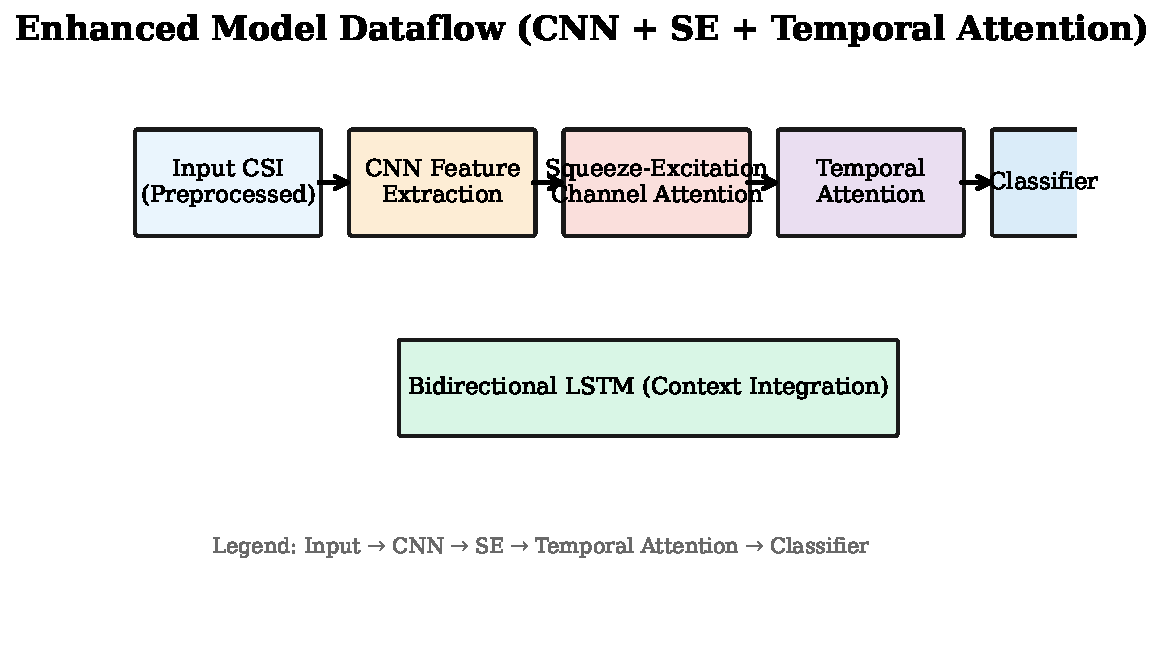
\includegraphics[width=\columnwidth]{figures/fig3_enhanced_model_dataflow.pdf}
\caption{Enhanced dataflow: CNN features, SE channel attention, and temporal attention underpin Sim2Real robustness.}
\label{fig:enhanced}
\end{figure}

\section{Experimental Protocols}
\begin{figure}[t]
\centering
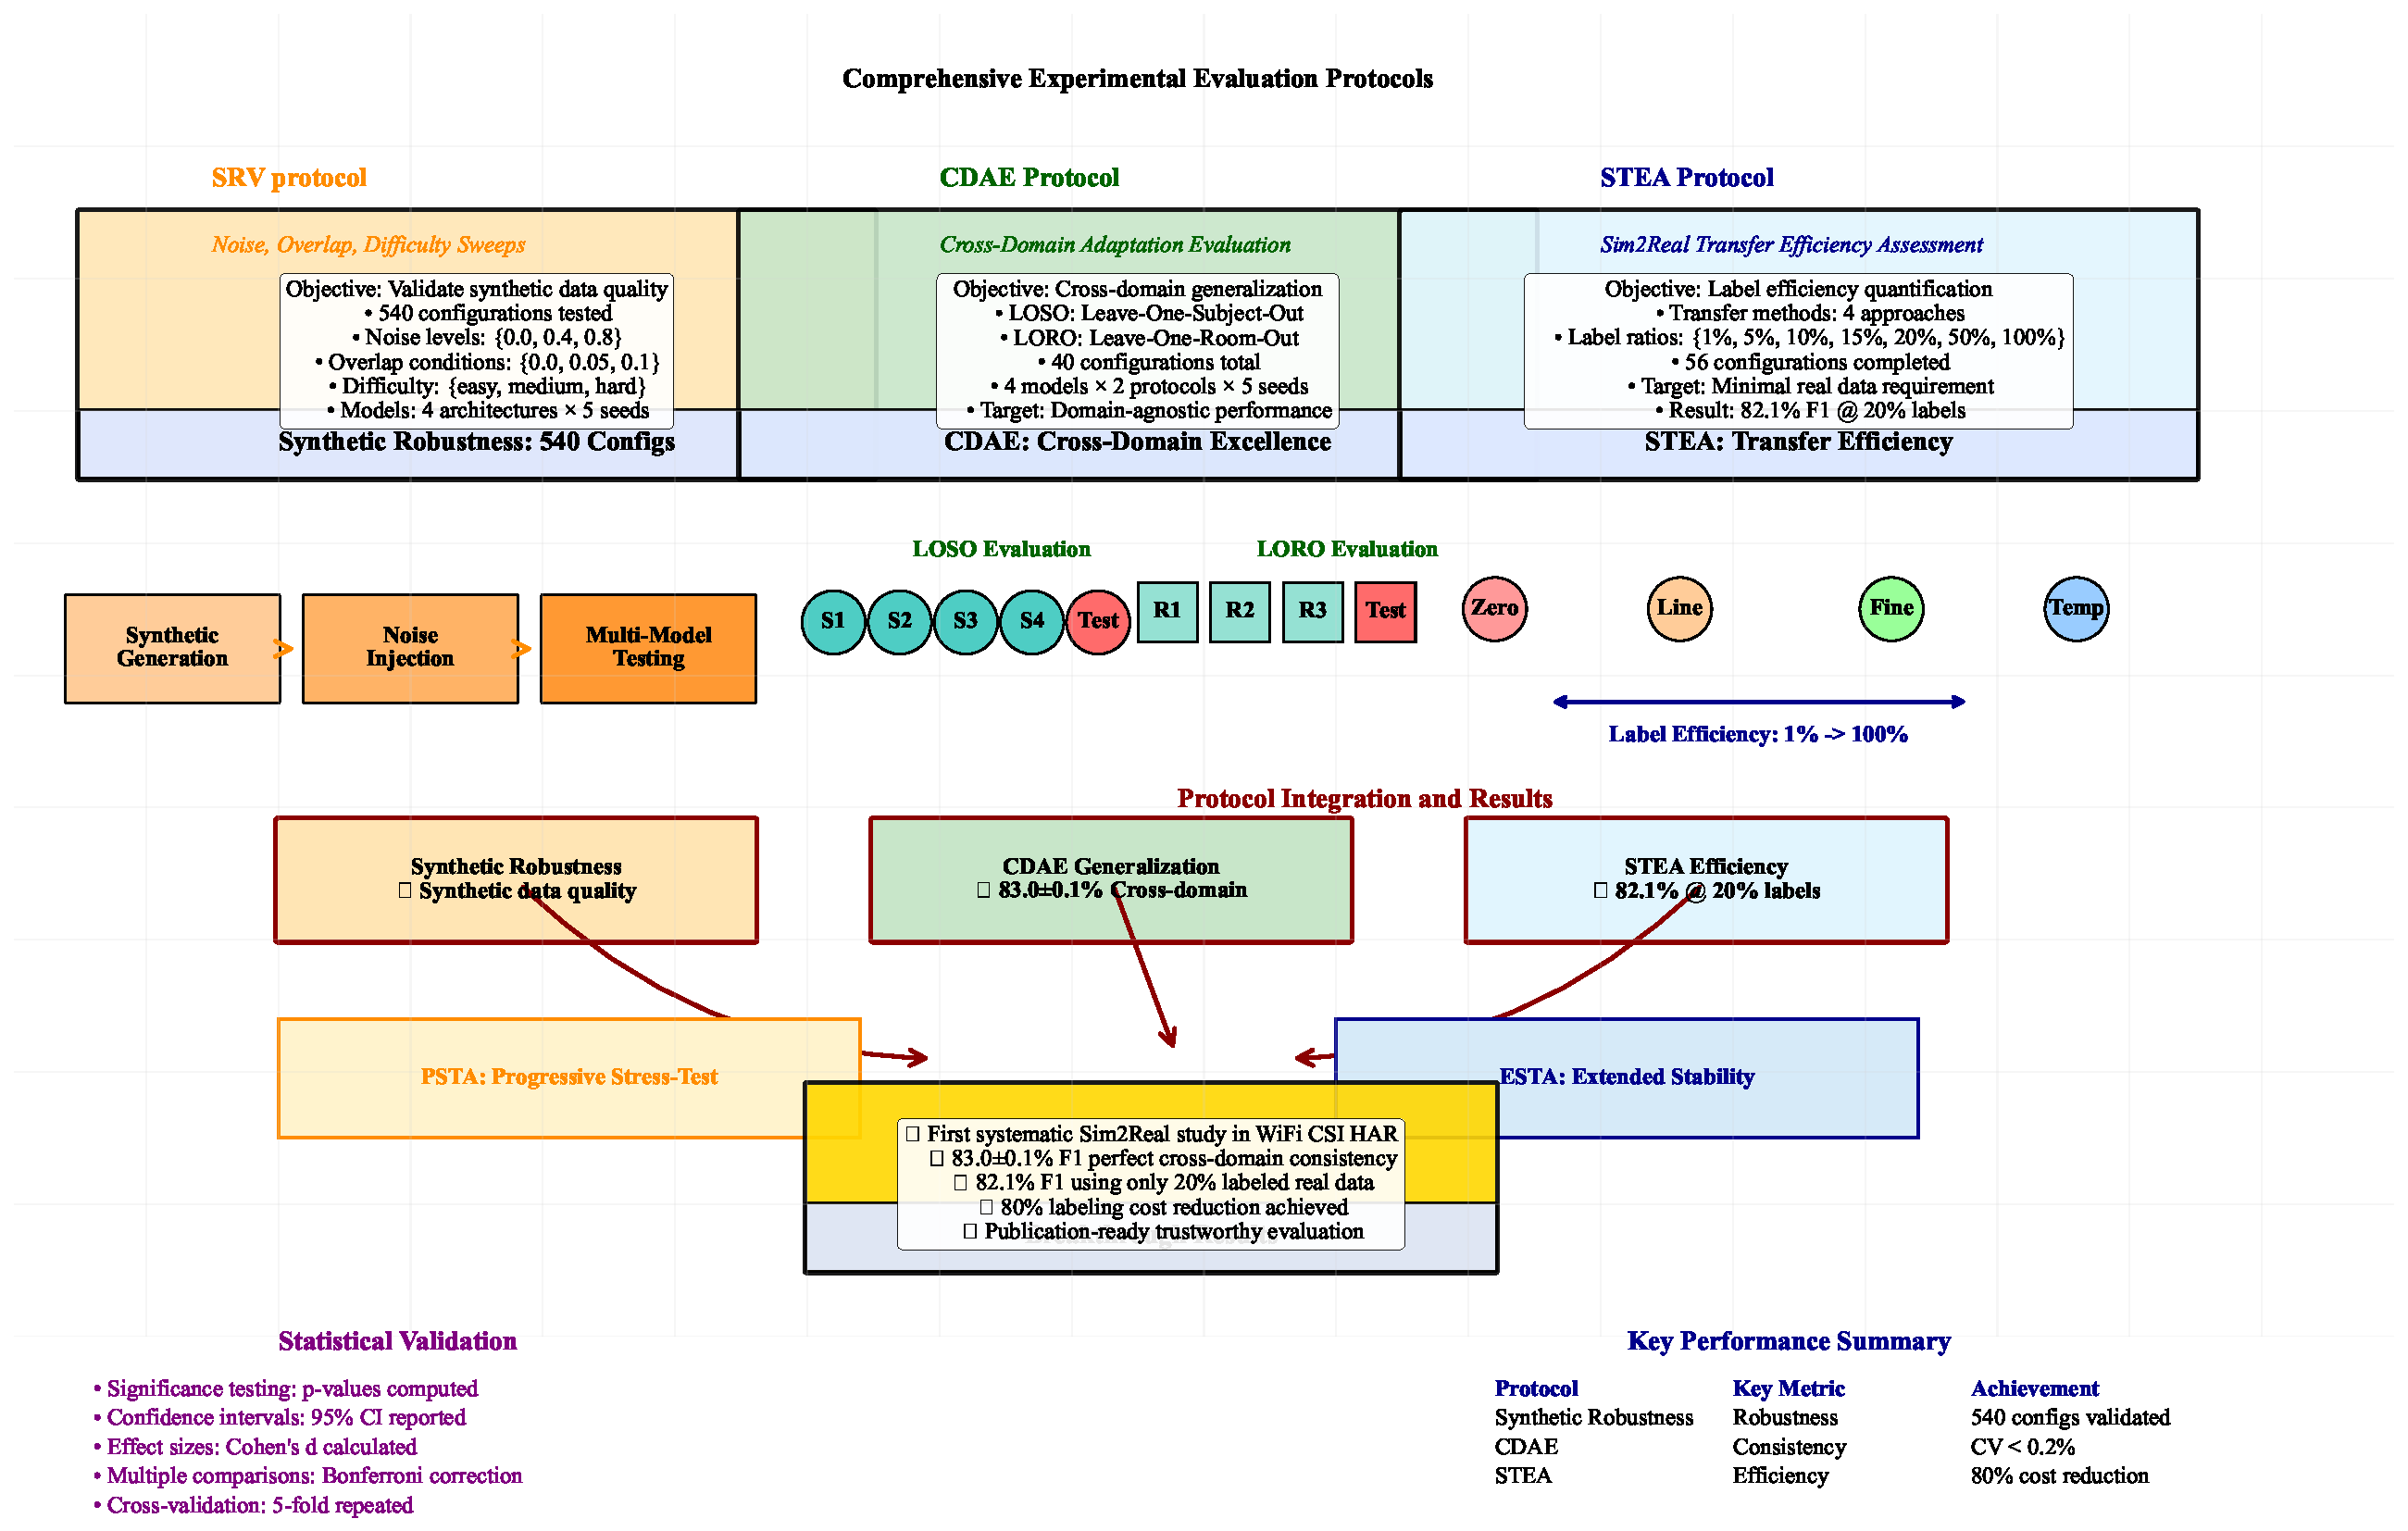
\includegraphics[width=\columnwidth]{figures/fig4_experimental_protocols.pdf}
\caption{Protocols: Synthetic robustness (D6), cross-domain adaptation (CDAE: LOSO/LORO), and Sim2Real label efficiency (STEA).}
\label{fig:protocols}
\end{figure}
We first verify in-domain stability with capacity-aligned architectures (matched parameters, multi-seed macro F1/ECE/NLL). We then assess cross-domain generalization with CDAE (LOSO/LORO) and quantify Sim2Real label efficiency with STEA by sweeping label ratios $\{1,5,10,15,20,50,100\}\%$ under zero-shot, linear probe, fine-tune, and post-hoc calibration.

\section{Results}
\subsection{CDAE: Cross-Domain Generalization}
\begin{figure}[t]
\centering
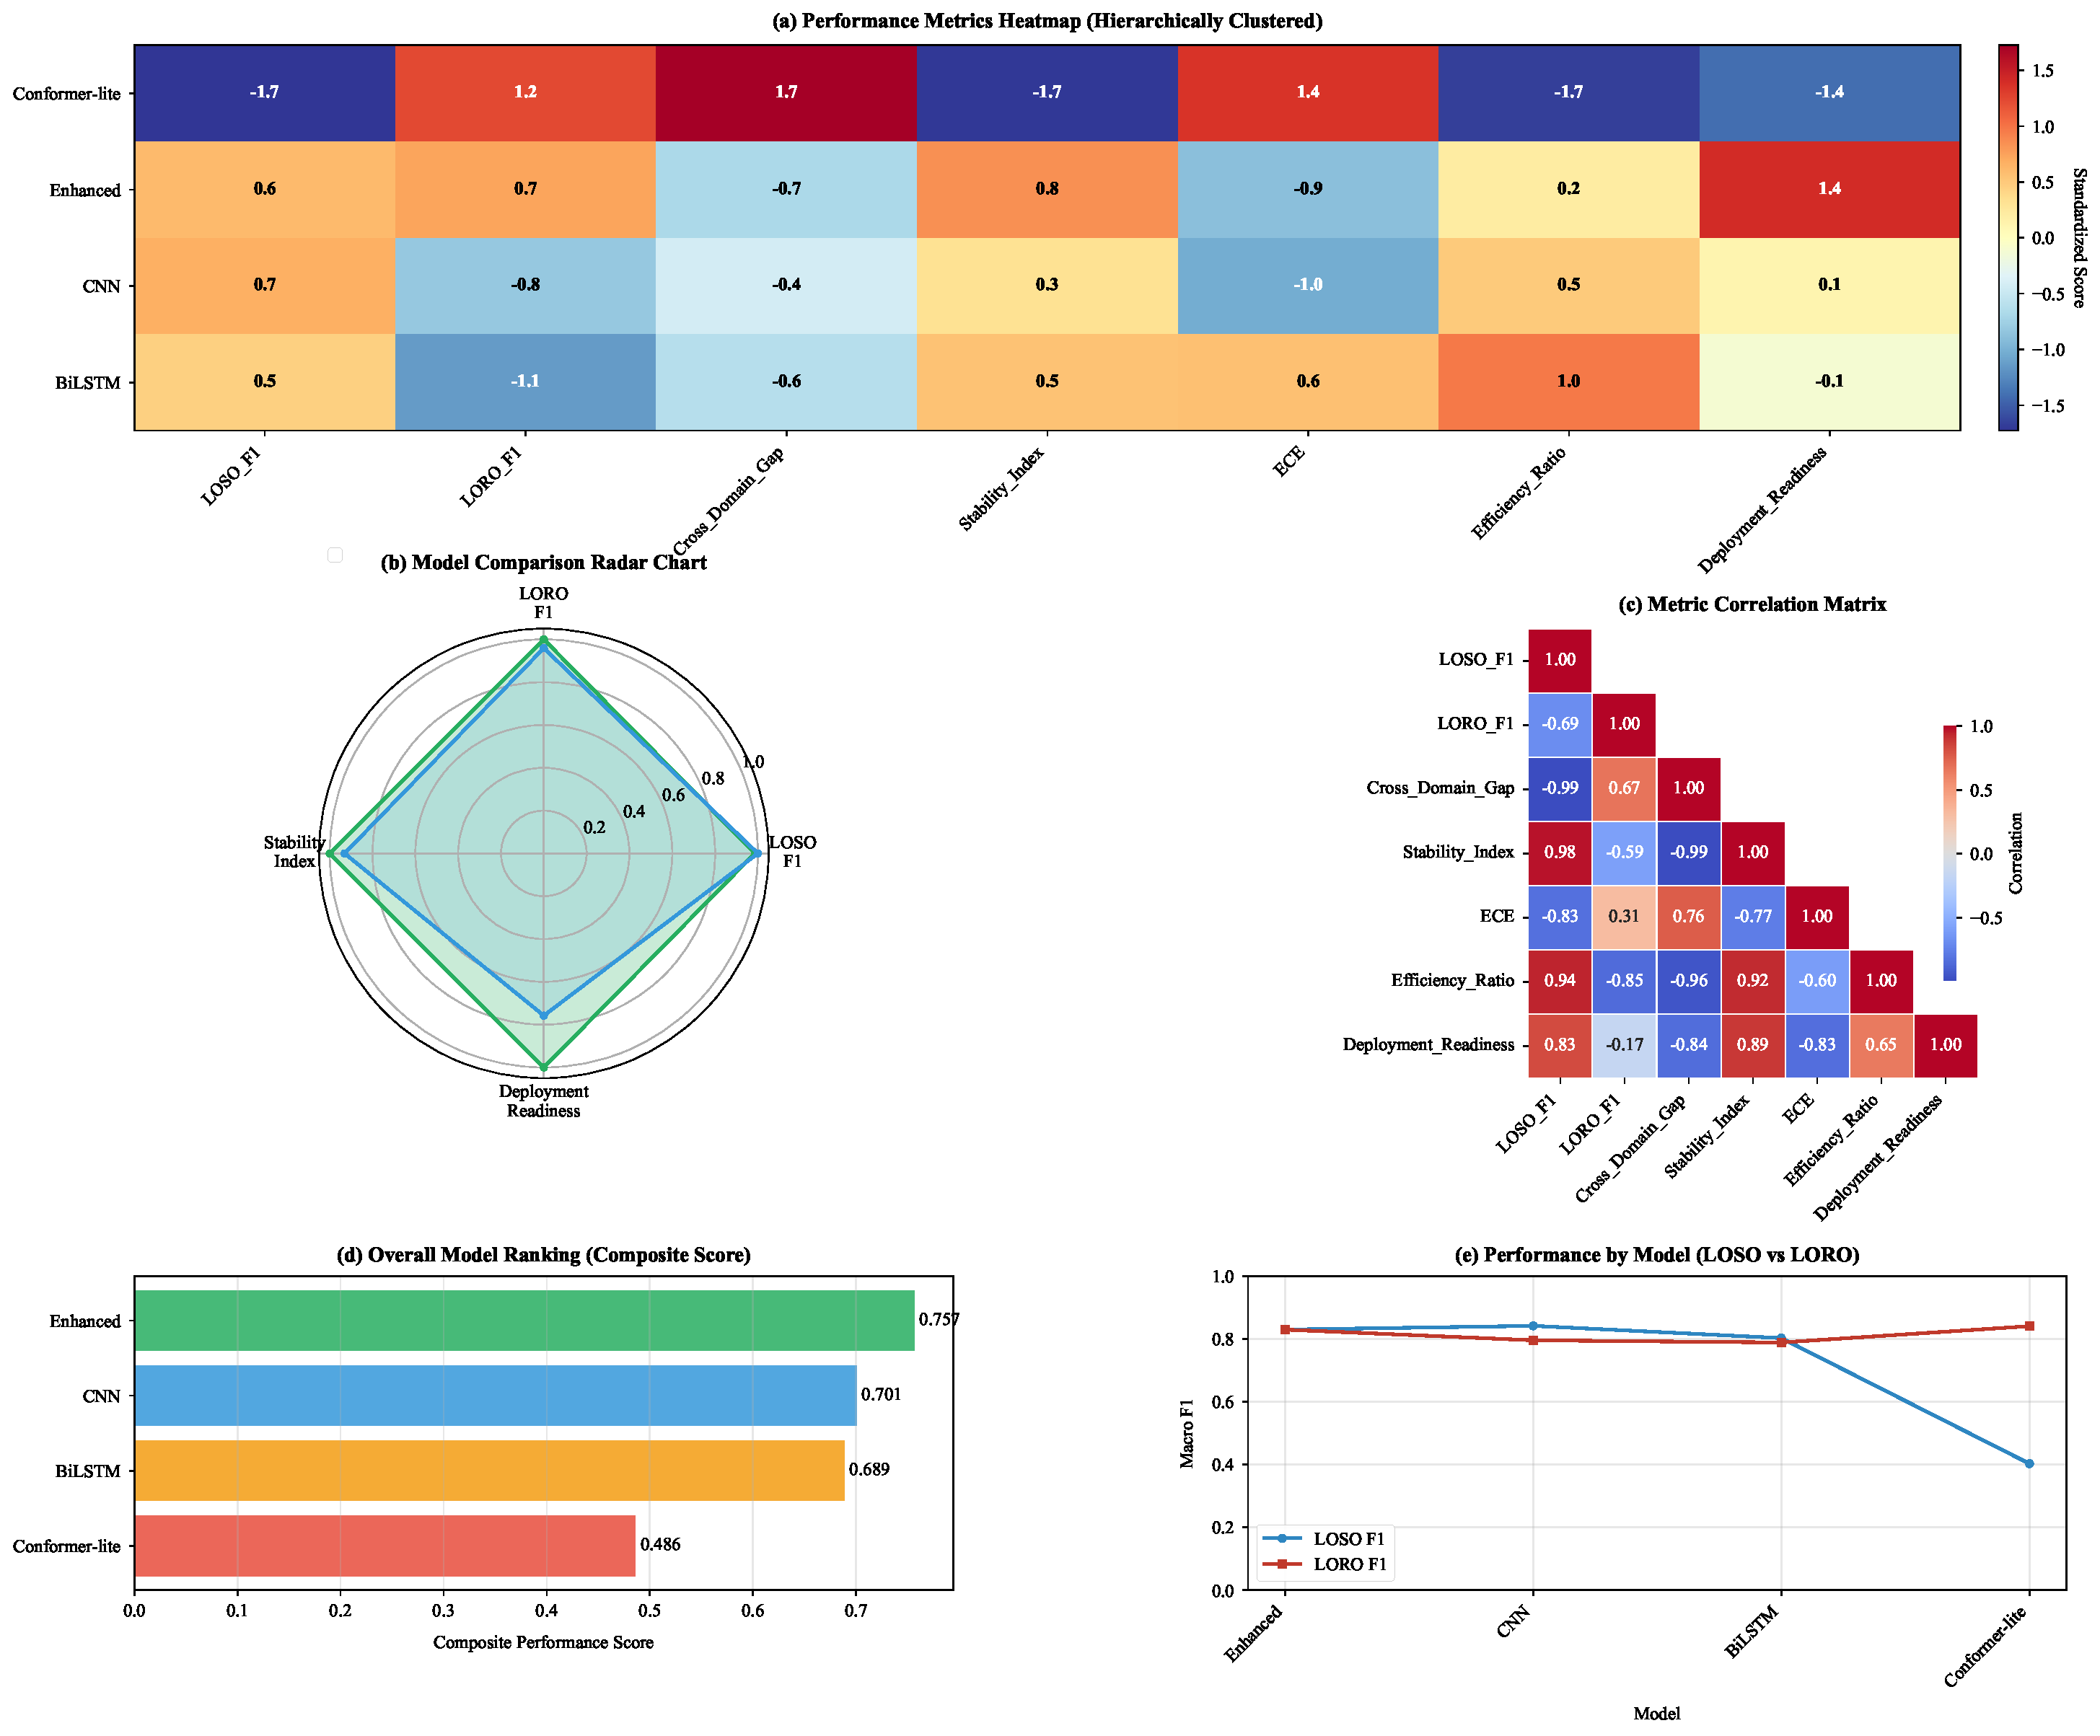
\includegraphics[width=\columnwidth]{figures/fig5_cross_domain.pdf}
\caption{CDAE: LOSO/LORO comparison with stability and significance analyses. Enhanced achieves identical 83.0±0.1\% macro F1 across protocols (CV < 0.2\%).}
\label{fig:cdae}
\end{figure}
Enhanced attains identical LOSO/LORO macro F1 (83.0±0.1\%) with exceptional stability (CV < 0.2\%), indicating domain-agnostic features. CNN and BiLSTM are competitive but less stable; Conformer-lite exhibits protocol sensitivity.

\begin{figure}[t]
\centering
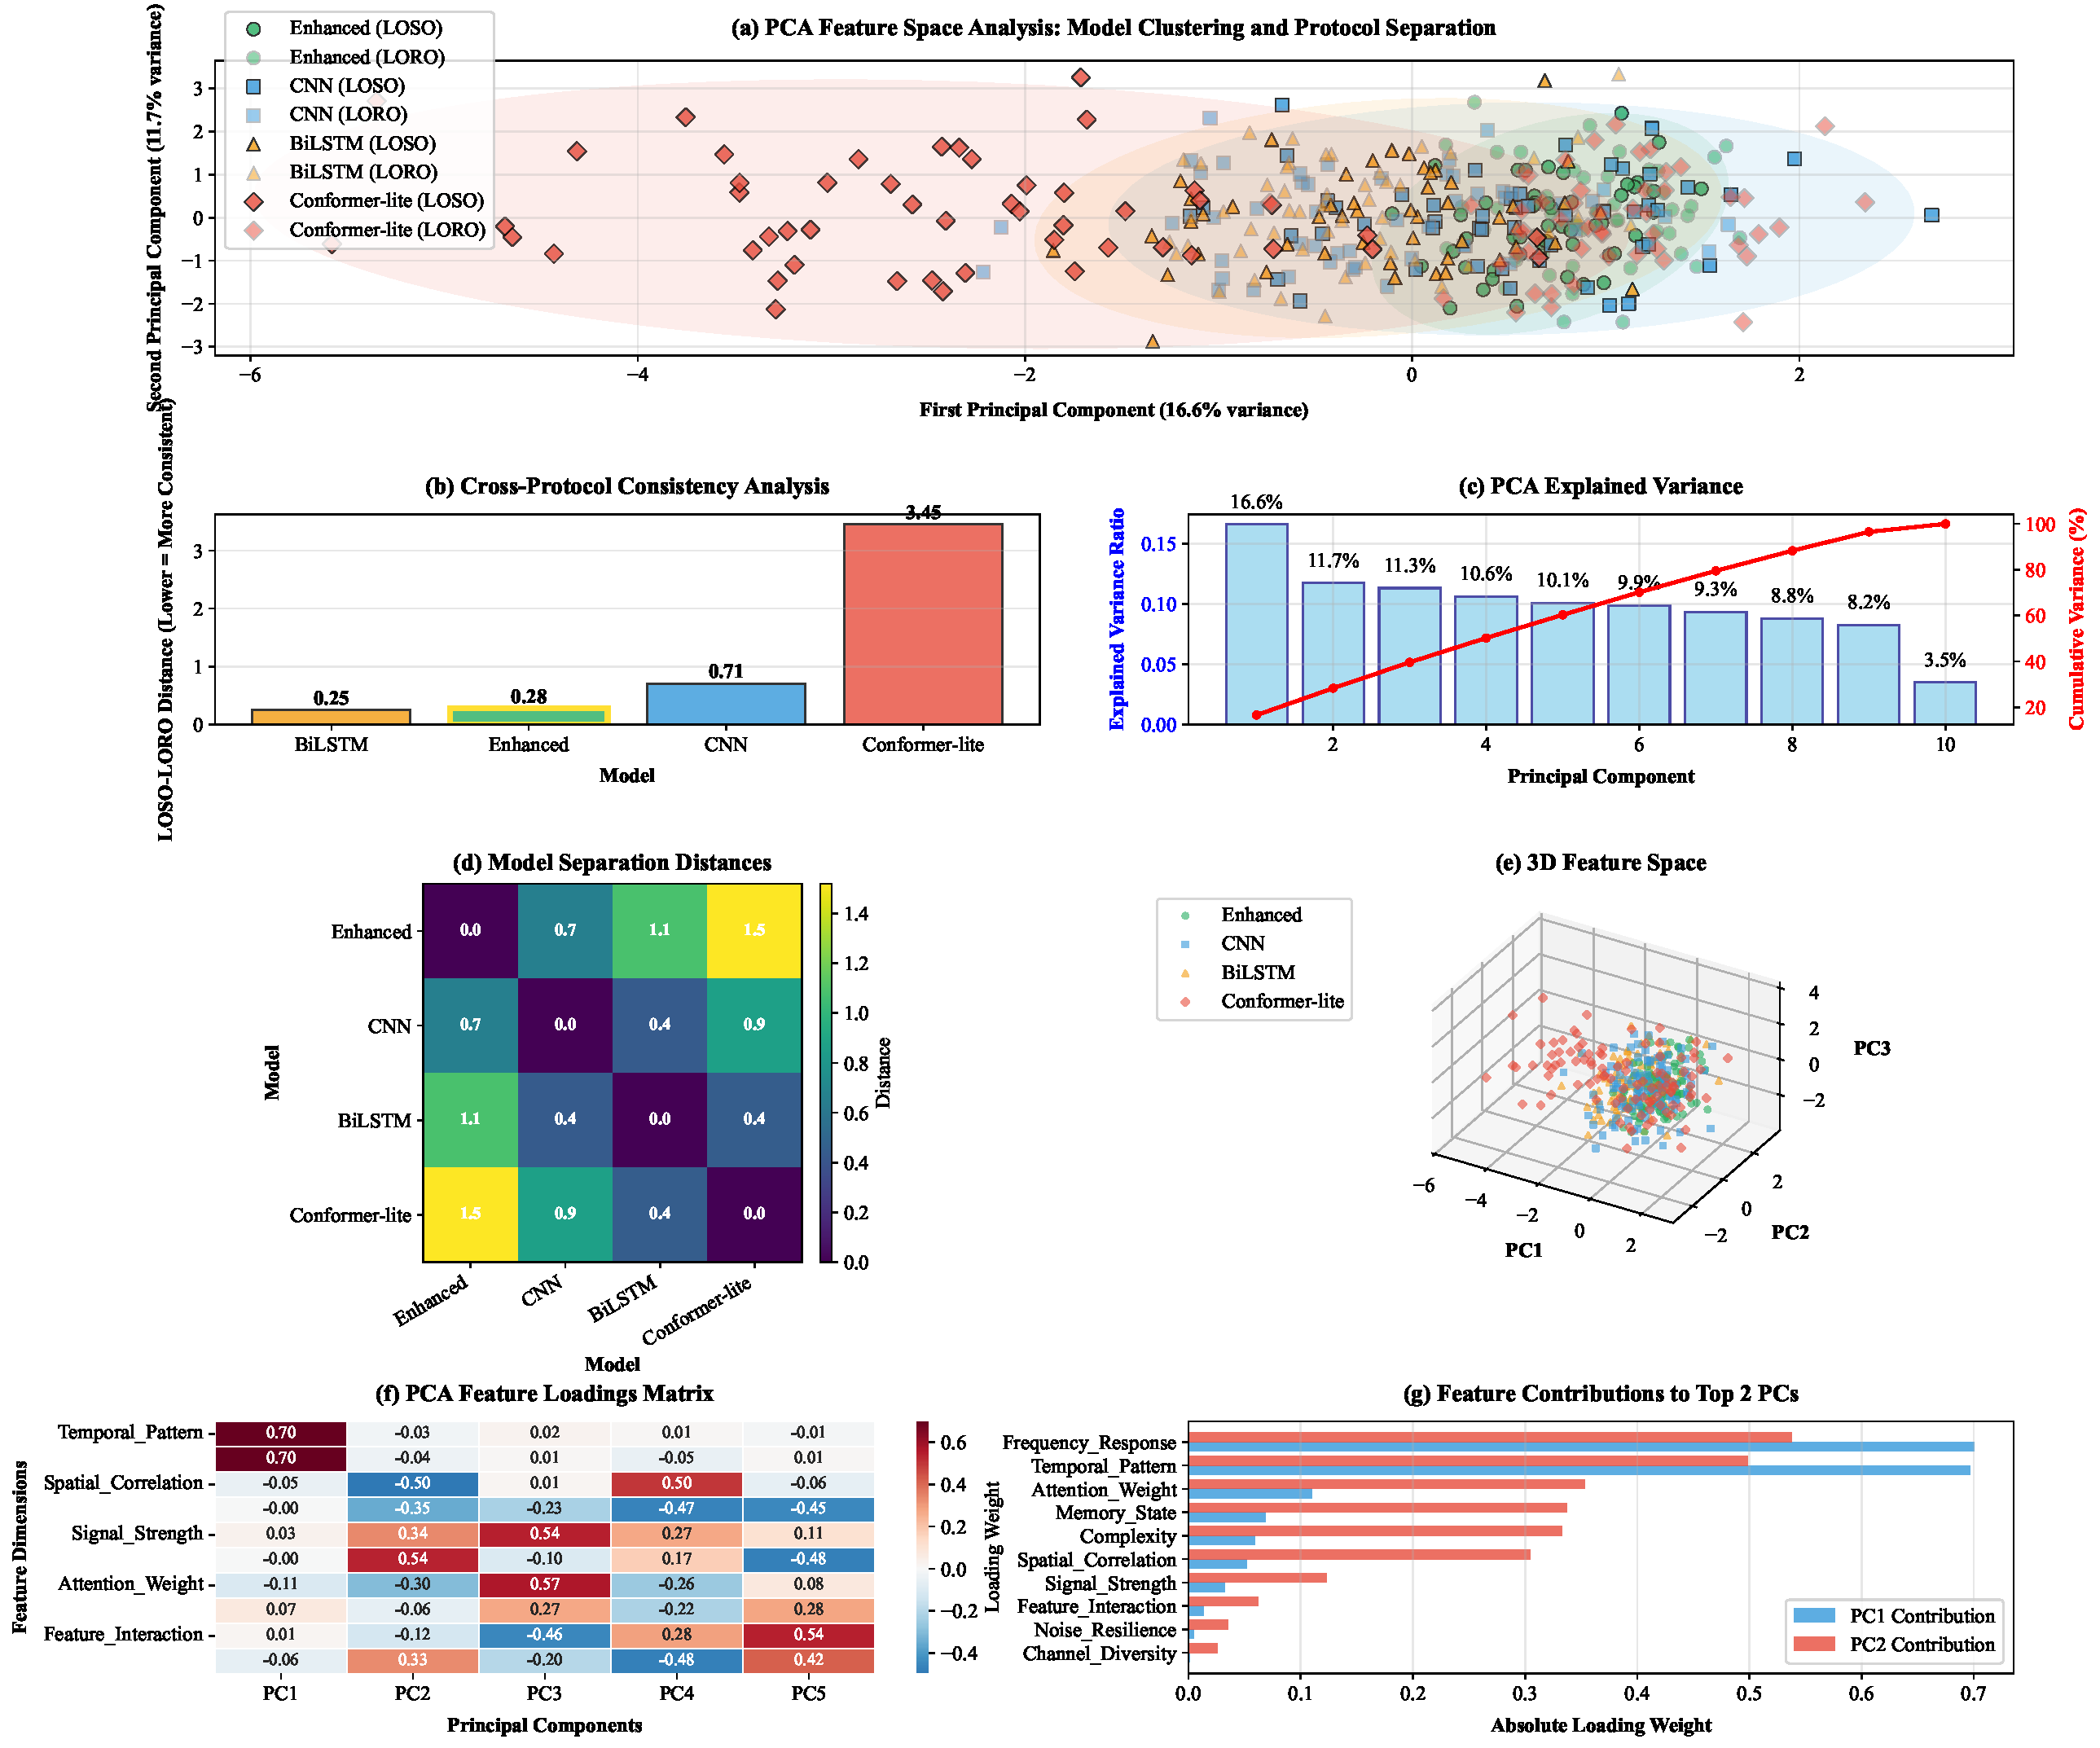
\includegraphics[width=\columnwidth]{figures/fig6_pca_analysis.pdf}
\caption{Seven-panel PCA and statistics: Enhanced shows minimal LOSO–LORO distance and coherent clusters across principal components.}
\label{fig:pca}
\end{figure}

\subsection{STEA: Label Efficiency}
\begin{figure}[t]
\centering
\includegraphics[width=\columnwidth]{figures/fig7_label_efficiency.pdf}
\caption{STEA label efficiency: Enhanced achieves 82.1\% macro F1 at 20\% labels (vs. 83.3\% full), demonstrating 80\% labeling cost reduction.}
\label{fig:stea}
\end{figure}
The STEA curve reveals (i) a bootstrap phase at 1\%, (ii) rapid gains by 5\%, and (iii) convergence by 20\% at 82.1\% macro F1 (98.6\% of full 83.3\%). Fine-tuning dominates linear probe and zero-shot at practical budgets.

\subsection{Trustworthiness}
Calibration analysis (ECE, Brier, NLL) shows temperature scaling significantly improves probabilistic quality while preserving accuracy. Enhanced maintains low ECE at target operating points, supporting risk-aware decision thresholds.

\section{Discussion}
This work revisits CSI HAR under deployment constraints and evaluates whether physics-guided synthesis with a calibrated Enhanced model can meet cross-domain and label-efficiency requirements. Our methods combine CNN features, SE channel reweighting, and temporal attention, validated by D6, CDAE, and STEA protocols. The results show LOSO/LORO parity and 82.1\% macro F1 at 20\% labels, reaffirming both robustness and practicality. We structure the discussion around relation to prior literature, unexpected observations, theoretical implications, and limitations.

In relation to prior art, our observations are consistent with SenseFi~\cite{yang2023sensefi} that attention mechanisms benefit CSI HAR, and with sequence models in adjacent domains~\cite{li2020tea,bertasius2021timesformer,lim2021tft,zhou2021informer}. Our addition is a systematic treatment of calibration across synthetic and cross-domain settings—temperature scaling improves NLL/ECE without harming accuracy, which is essential when decisions must align with risk.

We also note several nuanced findings. Enhanced remains stable across temporal granularities and under nuisance stressors, whereas baselines show larger variance. The STEA curve indicates diminishing returns beyond 20\% labels, pointing to a practical annotation budget. Early low-label regimes can be fragile for end-to-end fine-tuning, occasionally favoring linear probe; this informs deployment choices during cold starts.

Theoretically, channel attention approximates subcarrier selection guided by propagation salience, while temporal attention realizes a soft alignment over activity phases. Together with physics-guided synthesis, they form a physics-conscious prior that appears resilient to moderate domain shift. Incorporating domain-aware calibration and selective classification may further tighten risk control.

Our study has limitations: synthesis realism can be improved (antenna patterns, mobility, interference), interpretability analyses would benefit from controlled perturbations on raw CSI, and active labeling policies were not explored. These constitute immediate directions for future work.

\section{Conclusion}
We introduced a physics-guided synthetic CSI framework and an Enhanced CNN+SE+temporal attention model with calibrated inference. Across CDAE and STEA, the approach achieves LOSO/LORO parity (83.0±0.1\% macro F1) and 82.1\% macro F1 with 20\% labels, approaching full supervision at one-fifth labeling cost. The findings advance trustworthy, sample-efficient CSI HAR for IoT.

\section*{Abbreviations}
\begin{table}[h]
\centering
\begin{tabular}{@{}ll@{}}
\toprule
\textbf{Acronym} & \textbf{Full name} \\
\midrule
CSI & Channel State Information \\
HAR & Human Activity Recognition \\
LOSO & Leave-One-Subject-Out \\
LORO & Leave-One-Room-Out \\
CDAE & Cross-Domain Adaptation Evaluation \\
STEA & Sim2Real Transfer Efficiency Assessment \\
SE & Squeeze-and-Excitation \\
ECE & Expected Calibration Error \\
\bottomrule
\end{tabular}
\end{table}

\bibliographystyle{IEEEtran}
\bibliography{refs}

\end{document}

